\subsection{Layer 1 (Physical)}
\subsection*{Aufgaben}
\begin{itemize}
	\item Bits von A nach B bringen
	\item elektrische, mechanische oder andere physische Verbindung zwischen zwei Geräten
	\item Kodierung
\end{itemize}
\textbf{Geräte:} Kabel, Antenne, Hub, Repeater,...

\subsection*{Wichtige Begriffe}
\begin{itemize}
	\item Bandbreite (bits/s $\rightarrow$ theoretisch)
	\item Durchsatz (bits/s $\rightarrow$ praktisch)
	\item Latenz (Dauer der Daten von A bis B in ms)
\end{itemize}

\subsection*{Typische Medien}
\begin{itemize}
	\item Kupferkabel (Twisted-Pair-Kabel)
	\item[] \begin{tabbing}
		+ Günstig ~~~~~~~~~~~~~~~~~~~~~ \= $\approx$ Distanz (ca 100m) \\
		+ einfache Handhabung ~~~~ \= $\approx$ Geschwindigkeit \\
		~~~~~~~~~~~~~~~~~~~~~~~~~~~~~~~~~~~~ \= - Interferenzen (Störungen)
	\end{tabbing}
	\begin{itemize}
		\item Straight Through (beide Enden gleich)	
		\item Crossover (verschiedene Enden)
	\end{itemize}
	\item[] (durch Auto MDIX werden Enden automatisch konfiguriert)
	\item Koaxialkabel
	\item Glasfaserkabel
	\begin{tabbing}
		Arten: ~~ \= Single-Mode (Senden Laser, Reichweite 1-10km) \\
		~~~~~~~~~~~ \= Multi-Mode (Senden LED, Reichweite ca 600m)
	\end{tabbing}
	\item[] \begin{figure}[H]
		\centering
		\subfloat[\centering Single-Mode]{{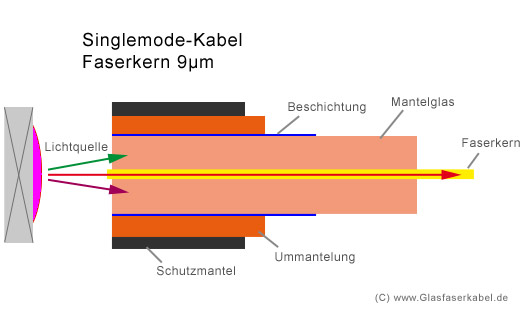
\includegraphics[width=0.46\linewidth]{figures/singlemode.jpg} }}
		\qquad
		\subfloat[\centering Multi-Mode]{{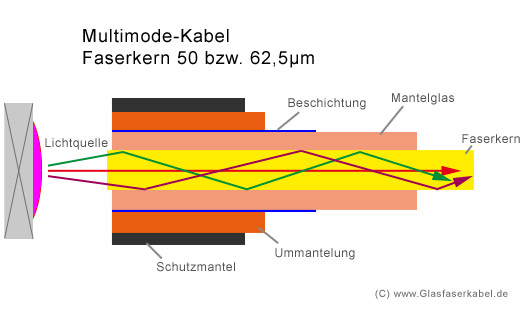
\includegraphics[width=0.46\linewidth]{figures/multimode.jpg} }}
		\caption{Glasfaserkabelarten}
	\end{figure}
	\item[] \begin{tabbing}
		+ Speed ~~~~~~~~~~~~~~~~~ \= - Teuer \\
		+ Reichweite ~~~~~~~~~~~ \= - Handhabung \\
		+ Störungen
	\end{tabbing}
	\item Drahtlos
	\item[] Übertragung: elektromagnetische Wellen über Luft
	\item[] \begin{tabbing}
		+ Flexibel ~~~ \= - Störungen \\
		~~~~~~~~~~~~~~~~~ \= - Shared Medium \\
		~~~~~~~~~~~~~~~~~ \= - Reichweite (ca 100m), Hindernisse \\
		~~~~~~~~~~~~~~~~~ \= - Security \\
	\end{tabbing}
\end{itemize}